\begin{frame}[hoved]
	\frametitle{Design}
	\begin{minipage}[t]{0.45\textwidth}
		{\large Requirements}
		\begin{itemize}
			\item Merge sort algorithm capable of running on a bare-metal RISC-V
			      processor.
			\item Capable of sorting lists of varying sizes.
		\end{itemize}
		{\large Bare-metal}
		\begin{itemize}
			\item Also known as Embedded system programming.
			\item Applications running without an underlying operating system.
			\item A lot of standard library implementations do not work out of the
			      box.
		\end{itemize}
	\end{minipage}
	\hfill
	\begin{minipage}[t]{0.45\textwidth}
		\begin{figure}
			\begin{center}
				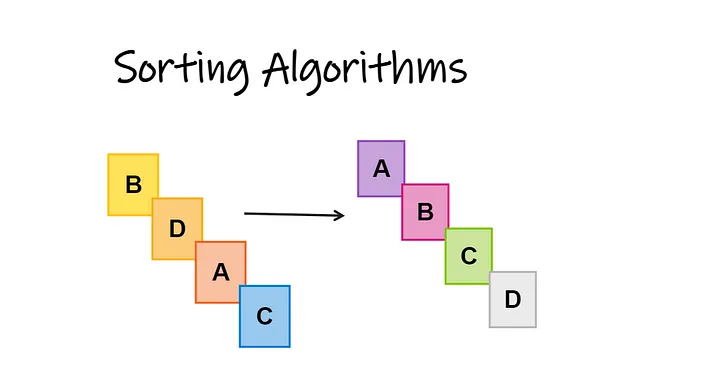
\includegraphics[width=0.95\textwidth]{figures/sorting.png}
			\end{center}
			\caption{\tiny https://medium.com/@noransaber685/understanding-sorting-algorithms-5575d52f5a18}\label{fig:}
		\end{figure}
	\end{minipage}
\end{frame}


\begin{frame}[hoved]
	\frametitle{Design}
	{\large Unikernel}
	\begin{itemize}
		\item Bridge between a fully fledge operating system and bare-metal.
		\item Allows a single application to run with some OS-support.
		\item Nanos. Meant for virtual machines only. An alternative to Docker with
		      Linux.
	\end{itemize}
	{\large freeRTOS}
	\begin{itemize}
		\item Real Time Operating System(RTOS).
		\item Gives some standard library functionality.
		\item Allows for more platform independent applications.
	\end{itemize}
	{\large Bare-metal}
	\begin{itemize}
		\item Processor uses RISC-V ISA with extensions:
		\item Control and Status Register(Zicsr), Atomic Instructions(a), Integer
		      Multiplication and Division (m), Compressed Instructions (c).
		\item Single vs multicore. Merge sort has a parallel structure. Parallel
		      should in theory increase performance.
	\end{itemize}
\end{frame}

\begin{frame}[hoved]
	\frametitle{Design}
	\begin{minipage}[t]{0.45\textwidth}
		{\large Scheduler vs Partitioning}
		\begin{itemize}
			\item Assuming cores have different execution speed, scheduler would allow
			      for the faster cores to do more.
			\item Scheduler would require synchronization.
			\item Partitioning makes each cores amount of work deterministic.
		\end{itemize}
	\end{minipage}
	\hfill
	\begin{minipage}[t]{0.45\textwidth}
		\begin{figure}
			\begin{center}
				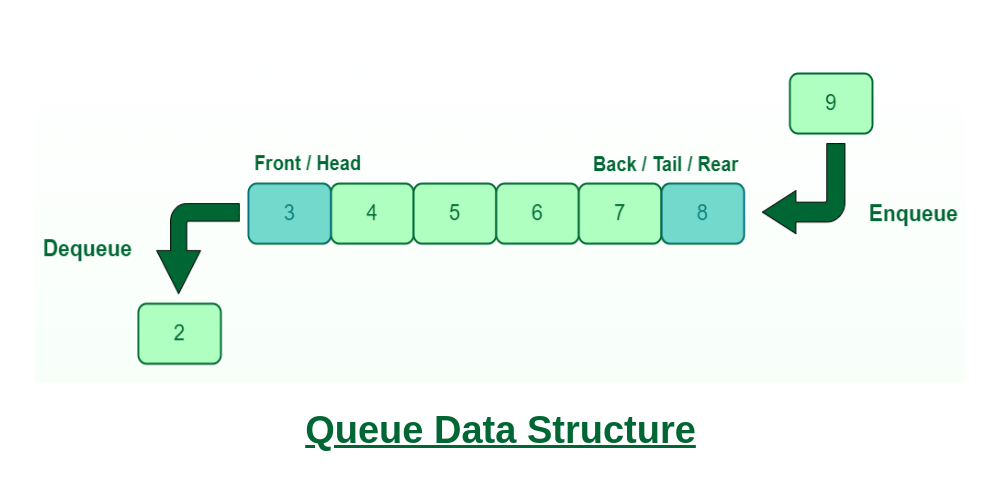
\includegraphics[width=0.95\textwidth]{figures/queue.png}
			\end{center}
			\caption{A queue data structure. \tiny https://www.geeksforgeeks.org/queue-meaning-in-dsa/}\label{fig:queue}
		\end{figure}
	\end{minipage}
\end{frame}

\begin{frame}[hoved]
	\frametitle{Design}
	\begin{minipage}[t]{0.45\textwidth}
		{\large Memory}
		\begin{itemize}
			\item Use context switching.
			\item Separate core memory and thread memory.
			\item When I had issues with corrupted data, I would have an idea of where
			      it was happening.
		\end{itemize}
		{\large Partitioning the list}
		\begin{itemize}
			\item Partition the list following the structure of the merge tree.
			\item Create threads for each level of the merge tree.
			\item Bottom level regular sort and not merge.
		\end{itemize}
	\end{minipage}
	\hfill
	\begin{minipage}[t]{0.45\textwidth}
		\begin{figure}
			\begin{center}
				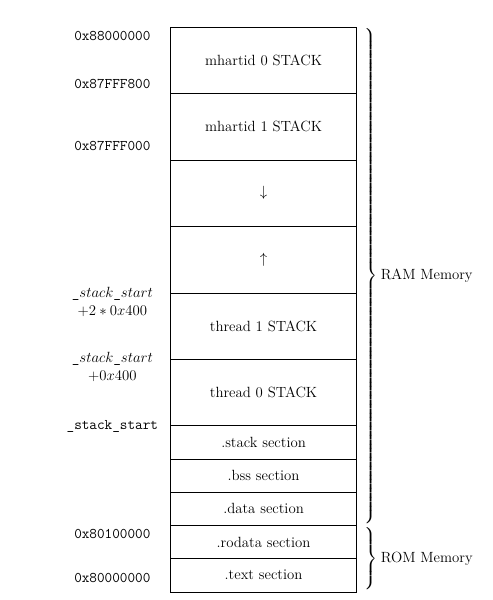
\includegraphics[height=0.65\textheight]{figures/memory.png}
			\end{center}
			\caption{Design of memory layout.}\label{fig:mem_layout}
		\end{figure}
	\end{minipage}
\end{frame}
